 %File: anonymous-submission-latex-2026.tex
\documentclass[a4, 10pt]{article} % DO NOT CHANGE THIS
% \usepackage[submission]{aaai2026}  % DO NOT CHANGE THIS
\usepackage{times}  % DO NOT CHANGE THIS
\usepackage{helvet}  % DO NOT CHANGE THIS
\usepackage{courier}  % DO NOT CHANGE THIS
\usepackage[hyphens]{url}  % DO NOT CHANGE THIS
\usepackage{graphicx} % DO NOT CHANGE THIS
\urlstyle{rm} % DO NOT CHANGE THIS
\def\UrlFont{\rm}  % DO NOT CHANGE THIS
\usepackage{natbib}  % DO NOT CHANGE THIS AND DO NOT ADD ANY OPTIONS TO IT
\usepackage{caption} % DO NOT CHANGE THIS AND DO NOT ADD ANY OPTIONS TO IT
\frenchspacing  % DO NOT CHANGE THIS
\setlength{\pdfpagewidth}{8.5in} % DO NOT CHANGE THIS
\setlength{\pdfpageheight}{11in} % DO NOT CHANGE THIS
%
% These are recommended to typeset algorithms but not required. See the subsubsection on algorithms. Remove them if you don't have algorithms in your paper.
\usepackage{algorithm}
\usepackage{algorithmic}
%
% Custom packages
\usepackage{amsmath}
\usepackage{amssymb}
\usepackage{booktabs}
\usepackage{subcaption}
\usepackage{pgfplots}
\usepackage{calc}
\usepackage{multirow}
\usepackage{tikz}
\usetikzlibrary{positioning,arrows.meta,backgrounds}
\pgfplotsset{compat=1.18}
\usepackage{tcolorbox}
\tcbuselibrary{breakable}
\newenvironment{pendingbox}[1][Pending experiment]{%
  \begin{tcolorbox}[colback=orange!8!white,colframe=orange!55!black,
    title={\small\bfseries #1},fonttitle=\small\bfseries,
    left=4pt,right=4pt,top=3pt,bottom=3pt,breakable]%
  \small\itshape}{%
  \end{tcolorbox}}
%
% These are are recommended to typeset listings but not required. See the subsubsection on listing. Remove this block if you don't have listings in your paper.
\usepackage{newfloat}
\usepackage{listings}
\DeclareCaptionStyle{ruled}{labelfont=normalfont,labelsep=colon,strut=off} % DO NOT CHANGE THIS
\lstset{%
	basicstyle={\footnotesize\ttfamily},% footnotesize acceptable for monospace
	numbers=left,numberstyle=\footnotesize,xleftmargin=2em,% show line numbers, remove this entire line if you don't want the numbers.
	aboveskip=0pt,belowskip=0pt,%
	showstringspaces=false,tabsize=2,breaklines=true}
\floatstyle{ruled}
\newfloat{listing}{tb}{lst}{}
\floatname{listing}{Listing}
%
% Keep the \pdfinfo as shown here. There's no need
% for you to add the /Title and /Author tags.
\pdfinfo{
/TemplateVersion (2026.1)
}


% DISALLOWED PACKAGES
% \usepackage{authblk} -- This package is specifically forbidden
% \usepackage{balance} -- This package is specifically forbidden
% \usepackage{color (if used in text)
% \usepackage{CJK} -- This package is specifically forbidden
% \usepackage{float} -- This package is specifically forbidden
% \usepackage{flushend} -- This package is specifically forbidden
% \usepackage{fontenc} -- This package is specifically forbidden
% \usepackage{fullpage} -- This package is specifically forbidden
% \usepackage{geometry} -- This package is specifically forbidden
% \usepackage{grffile} -- This package is specifically forbidden
% \usepackage{hyperref} -- This package is specifically forbidden
% \usepackage{navigator} -- This package is specifically forbidden
% (or any other package that embeds links such as navigator or hyperref)
% \indentfirst} -- This package is specifically forbidden
% \layout} -- This package is specifically forbidden
% \multicol} -- This package is specifically forbidden
% \nameref} -- This package is specifically forbidden
% \usepackage{savetrees} -- This package is specifically forbidden
% \usepackage{setspace} -- This package is specifically forbidden
% \usepackage{stfloats} -- This package is specifically forbidden
% \usepackage{tabu} -- This package is specifically forbidden
% \usepackage{titlesec} -- This package is specifically forbidden
% \usepackage{tocbibind} -- This package is specifically forbidden
% \usepackage{ulem} -- This package is specifically forbidden
% \usepackage{wrapfig} -- This package is specifically forbidden
% DISALLOWED COMMANDS
% \nocopyright -- Your paper will not be published if you use this command
% \addtolength -- This command may not be used
% \balance -- This command may not be used
% \baselinestretch -- Your paper will not be published if you use this command
% \clearpage -- No page breaks of any kind may be used for the final version of your paper
% \columnsep -- This command may not be used
% \newpage -- No page breaks of any kind may be used for the final version of your paper
% \pagebreak -- No page breaks of any kind may be used for the final version of your paperr
% \pagestyle -- This command may not be used
% \tiny -- This is not an acceptable font size.
% \vspace{- -- No negative value may be used in proximity of a caption, figure, table, section, subsection, subsubsection, or reference
% \vskip{- -- No negative value may be used to alter spacing above or below a caption, figure, table, section, subsection, subsubsection, or reference

\setcounter{secnumdepth}{0} %May be changed to 1 or 2 if section numbers are desired.

% The file aaai2026.sty is the style file for AAAI Press
% proceedings, working notes, and technical reports.
%

% Title

% Your title must be in mixed case, not sentence case.
% That means all verbs (including short verbs like be, is, using,and go),
% nouns, adverbs, adjectives should be capitalized, including both words in hyphenated terms, while
% articles, conjunctions, and prepositions are lower case unless they
% directly follow a colon or long dash
\title{DEEP-MIRT: Dynamic Psychometric Knowledge Tracing for Partial-Credit and Rubric-Scored Assessment}
\author{
    %Authors
    % All authors must be in the same font size and format.
    Wenrui Yuan,
    St\'{e}phanie van den Berg,
    Johannes Steinr\"{u}cke
}
% \affiliations{
%     %Afiliations
%     \textsuperscript{\rm 1}Association for the Advancement of Artificial Intelligence\\
%     % If you have multiple authors and multiple affiliations
%     % use superscripts in text and roman font to identify them.
%     % For example,

%     % Sunil Issar\textsuperscript{\rm 2},
%     % J. Scott Penberthy\textsuperscript{\rm 3},
%     % George Ferguson\textsuperscript{\rm 4},
%     % Hans Guesgen\textsuperscript{\rm 5}
%     % Note that the comma should be placed after the superscript

%     1101 Pennsylvania Ave, NW Suite 300\\
%     Washington, DC 20004 USA\\
%     % email address must be in roman text type, not monospace or sans serif
%     proceedings-questions@aaai.org
% %
% % See more examples next
% }

% %Example, Single Author, ->> remove \iffalse,\fi and place them surrounding AAAI title to use it
% \iffalse
% \title{My Publication Title --- Single Author}
% \author {
%     Author Name
% }
% \affiliations{
%     Affiliation\\
%     Affiliation Line 2\\
%     name@example.com
% }
% \fi

% \iffalse
% %Example, Multiple Authors, ->> remove \iffalse,\fi and place them surrounding AAAI title to use it
% \title{My Publication Title --- Multiple Authors}
% \author {
%     % Authors
%     First Author Name\textsuperscript{\rm 1},
%     Second Author Name\textsuperscript{\rm 2},
%     Third Author Name\textsuperscript{\rm 1}
% }
% \affiliations {
%     % Affiliations
%     \textsuperscript{\rm 1}Affiliation 1\\
%     \textsuperscript{\rm 2}Affiliation 2\\
%     firstAuthor@affiliation1.com, secondAuthor@affilation2.com, thirdAuthor@affiliation1.com
% }
% \fi


% % REMOVE THIS: bibentry
% % This is only needed to show inline citations in the guidelines document. You should not need it and can safely delete it.
% \usepackage{bibentry}
% END REMOVE bibentry

\begin{document}

\maketitle

\begin{abstract}
Knowledge tracing is a core component of adaptive learning systems, yet much of the literature assumes binary correctness as the observation signal. In many educational settings, however, learner evidence is polytomous, including ordered rubric levels and partial credit, where both ordinal structure and interpretability matter for measurement and intervention. 

We present DEEP-MIRT, a modular framework that extends knowledge tracing to polytomous responses by bridging sequential neural modeling with psychometric Item Response Theory. The framework couples a swappable sequential backbone with an interchangeable IRT-grounded response head, separating the question of how learner ability evolves over time from the question of how that ability maps to ordered response categories. Instantiated with a Generalized Partial Credit Model (GPCM) head, DEEP-MIRT produces interpretable outputs at every interaction: an evolving student ability estimate, per-item discrimination values, and ordered difficulty thresholds corresponding to rubric level transitions. On synthetic benchmarks with known ground truth, DEEP-GPCM achieves strong rank-order agreement across category resolutions $K\in\{2,3,4,5\}$ (QWK up to 0.778) and recovers item difficulty thresholds and discrimination with high to moderate fidelity (mean $r_{\beta}=0.90$; $r_{\alpha}\approx 0.65$). The model remains backward-compatible with standard binary knowledge tracing benchmarks, matching established baselines on ASSIST2015 and Synthetic-5 with $K=2$. Together, the proposed model advances knowledge tracing from a binary predictive instrument into a measurement-aware framework that supports both instructional decision-making with psychometric interpretation.
\end{abstract}



\section{Introduction}
Educational assessments often target graded performance rather than pass/fail outcomes. Rubric-based scoring, partial-credit items, and constructed-response tasks encode degrees of correctness that binary labels collapse into a single signal \citep{black_assessment_1998, heritage_formative_2007}.
While automated scoring systems can deliver this ordinal structure at scale in intelligent tutoring contexts \citep{shute_stealth_2011, baral_improving_2021}, most KT benchmarks, evaluation protocols, and dominant modeling paradigms still assume binary correctness. This leaves ordinal outcomes comparatively underexplored in KT, even though they are central to authentic assessment practice.

% Knowledge Tracing (KT) is central to adaptive instruction in Intelligent Tutoring Systems (ITS) and online learning platforms: from a learner’s interaction history, a KT model estimates an evolving latent knowledge state to support feedback, practice selection, and mastery decisions \citep{aleven_embedding_2016}. For educational use, KT must be accurate and interpretable to support assessment arguments, teacher trust, and curriculum integration.

Beyond the outcome type, interpretability remains a key concern. Most KT models learn high-dimensional states optimized for prediction, but these states are not, by construction, tied to interpretable quantities. Therefore, constructs that educators and assessment designers routinely work with, such as student ability level, item discriminatory power, or the difficulty steps between adjacent rubric categories, are not directly identifiable. Item Response Theory (IRT) provides exactly this structure through identifiable parameters including student ability, item discrimination, and ordered step difficulties, grounding score interpretation in established psychometric theory \citep{van_der_linden_generalized_1997, embretson_irt_2000, messick_validity_1995}. Standard IRT models, however, treat ability as fixed and are not designed for sequential interaction data. This work therefore extends KT to polytomous responses by incorporating the interpretable parameter structure of IRT within a dynamic sequential framework.

% The majority of KT research, however, relies on binary states to represent mastery levels. This is a lossy observation model for many learning interactions that are naturally \emph{polytomous}, such as rubric scores, multi-step problems with partial credit, attempts/hints/time-to-solve signals, nominal multiple-choice distractions that encode different misconceptions, multi-response items, and ranking/ordering tasks. Collapsing these signals into a binary label loses details for formative assessment that are central to learning progressions.

Three lines of existing work address these issues in isolation, leaving a gap at their intersection. First, deep KT models, from Deep Knowledge Tracing \citep[DKT;][]{piech_deep_2015} to memory-augmented and attention-based variants \citep{zhang_dynamic_2017, pandey_self-attentive_2019}, capture temporal learning dynamics but typically assume dichotomous correctness and learn latent states with limited psychometric interpretability. Second, polytomous Item Response Theory (IRT) models such as the Generalized Partial Credit Model \citep[GPCM;][]{van_der_linden_generalized_1997} provide principled, interpretable measurement of ordered responses with identifiable parameters (student ability, item discrimination, ordered step thresholds), but they generally treat ability as time-invariant and are not designed for sequential interaction logs. Third, recent efforts that inject IRT structure into deep KT \citep{yeung_deep-irt_2019, converse_irt_kt_2021} improve interpretability but largely remain restricted to dichotomous outcomes. An early partial exception is \citet{wang_extending_2013}, who extended Bayesian Knowledge Tracing to allow partial credit via continuous Bayesian nodes, but without deep sequential modeling or recovering standard polytomous IRT step structure. Yet these approaches has not yet reconciled sequential dynamics with ordinal response modeling while retraining psychometric identifiability.

We propose \textit{DEEP-MIRT}, a modular framework that extends KT to Polytomous Knowledge Tracing (PKT) by coupling a swappable sequential backbone with an IRT-grounded response head. In this setting, PKT is the task of predicting the full distribution over ordered response categories from a learner’s interaction history. We instantiate the framework with a GPCM response head, yielding DEEP-GPCM, which combines a Dynamic Key-Value Memory Network (DKVMN) backbone with a GPCM observation model. At each timestep, the GPCM head maps the learner state to a distribution over ordinal categories and exposes psychometrically interpretable components, including an evolving student ability estimate, as well as learned item parameters such as per-item discrimination values and ordered step difficulties corresponding to rubric level transitions. While the experiments focus on ordinal PKT, the framework accommodates other polytomous formats through alternative response heads.

% We refer to this broader problem family as \textit{Polytomous Knowledge Tracing (PKT)}: given an interaction history $\mathcal{X}_t=\{x_1,\ldots,x_t\}$ with $x_t=(q_t,r_t)$, the goal is to predict the distribution of the next response $P(r_{t+1}\mid q_{t+1},\mathcal{X}_t)$, where the response space depends on the item format (ordered categories for partial credit; unordered options for multiple choice; sets for multi-response; permutations for ranking). Particularly, we focus on the most common PKT setting in assessment and tutoring: \textit{ordinal} responses with $r_t\in\{0,1,\ldots,K-1\}$ and prediction target $P(r_{t+1}=k\mid q_{t+1},\mathcal{X}_t)$ for each ordered category $k$.

% A core challenge in student modeling is to reconcile \textit{static measurement} with \textit{dynamic state evolution}: psychometric models provide identifiable and interpretable measurement, but are typically static; deep sequential KT models capture temporal dynamics, but are weakly constrained and hard to interpret. This challenge is amplified for PKT because deep KT is largely organized around binary correctness, making multi-category outcomes harder to model. Recent KT work has also highlighted that problem complexity and unstable knowledge state updates can deteriorate predictive performances \citep{li_pskt_2025}, and that rich process features (e.g., attempts and response time) contain information beyond correctness \citep{lu_selfkt_2024}. PKT therefore calls for models that are simultaneously dynamic, format-aware, and psychometrically interpretable.

% We propose \textit{DEEP-MIRT} as a \emph{framework} for extending dichotomous KT to PKT by coupling a swappable sequential backbone (e.g., memory networks or attention) with a \emph{response-aware head} grounded in psychometric item response models. In this study, we instantiate the framework for ordinal/partial-credit responses via a Generalized Partial Credit Model (GPCM) head, yielding two showcase models: \textbf{DEEP-GPCM}, which combines a DKVMN-style dynamic memory with a GPCM observation model, and \textbf{ATTN-GPCM}, which further integrates self-attention mechanisms to improve interaction representation and memory addressing. While our experiments emphasize ordinal PKT, the framework is designed to accommodate other polytomous formats (e.g., nominal multiple-choice and ranking) through alternative response heads.

Our main contributions are:
\begin{enumerate}
    \item \textbf{A modular framework for polytomous knowledge tracing.} We formulate PKT as predicting the full ordinal response distribution from interaction history and propose DEEP-MIRT, which decouples a sequential backbone (encoder, memory, summary) from an interchangeable psychometric response head. The head interface accepts student ability $\theta_t$ and item identity $\mathbf{k}_t$ and returns a category probability vector; any differentiable observation model satisfying this contract is a valid instantiation. This design separates the educational measurement question (which model governs how ability maps to rubric scores?) from the knowledge tracing question (how does ability evolve over time?).
    \item \textbf{GPCM instantiation with interpretable psychometric parameters.} We instantiate DEEP-MIRT with a GPCM-based response head as DEEP-GPCM, incorporating a monotonic threshold parameterization that enforces rubric ordering by construction. The resulting model produces evolving ability trajectories, item discrimination estimates, and ordered step difficulty thresholds, all of which correspond to constructs that educators and assessment designers already use in rubric design and standard-setting practice.
    \item \textbf{Scalable item encoding and empirical evaluation.} We propose Static Item Embedding (SIE) for large item banks and evaluate ordinal prediction quality, psychometric parameter recovery, ablation of design components, and backward compatibility with binary KT benchmarks.
\end{enumerate}

We investigate the following research questions:
\begin{itemize}
    \item \textbf{RQ1 (Prediction).} Does coupling a DKVMN backbone with an ordinal, psychometrically-constrained GPCM response head improve polytomous next-response prediction, and does it better preserve ordinal structure than format-unaware alternatives?
    \item \textbf{RQ2 (Parameter Recovery).} Do the IRT parameters inferred by DEEP-GPCM faithfully recover known ground-truth values from synthetic data, and are item parameter estimates stable across student subpopulations as assessed by split-half reliability?
    \item \textbf{RQ3 (Learner State).} Do the inferred student ability trajectories $\theta_t$ exhibit psychologically plausible learning dynamics, and can DEEP-GPCM reveal meaningful learner patterns (mastery, growth, persistent difficulty) that are not visible from format-unaware latent state representations?
    \item \textbf{RQ4 (Scalability).} Does Static Item Embedding maintain ordinal prediction quality and parameter recovery at large item-bank scales ($Q \sim 5{,}000$) while substantially reducing parameter count compared to dense encoding strategies?
    \item \textbf{RQ5 (Ecological Validity).} When ordinal response categories are constructed from proxy signals in existing binary KT benchmarks (e.g., attempt counts), does the ordinal GPCM head yield measurable gains over format-unaware alternatives, and how sensitive are these gains to the quality of the proxy ordinal construction?
\end{itemize}


\section{Related Work}
\subsection{Knowledge Tracing: From Binary to Polytomous}
Knowledge tracing has evolved through several modeling paradigms, but all share a common assumption: learner responses are binary. Bayesian Knowledge Tracing (BKT) models mastery of a Knowledge Component (KC) as a two-state Hidden Markov Model \citep{corbett_knowledge_1994}. Deep Knowledge Tracing (DKT) reframed the task as sequence modeling with recurrent neural networks, learning high-dimensional latent states from interaction sequences \citep{piech_deep_2015}. Dynamic Key-Value Memory Networks (DKVMN) introduced a structured memory that separates static concept representations (key memory) from evolving mastery states (value memory), offering a more transparent mapping between knowledge components and latent state than generic RNNs \citep{graves_hybrid_2016, zhang_dynamic_2017}. Attention-based models such as SAKT and AKT apply self-attention to weigh the relevance of prior interactions for next-step prediction \citep{pandey_self-attentive_2019, ghosh_context-aware_2020}, and recent work has further explored Transformer-based architectures \citep{choi_saint_2020, liu_simplekt_2023}. Throughout this progression, the response format has remained dichotomous: every model cited above predicts a binary correct/incorrect outcome.

Recent KT research has begun to acknowledge that correctness alone is insufficient. \citet{lu_selfkt_2024} fuse process features (attempts, response time, historical accuracy) to enrich difficulty representations, and \citet{li_pskt_2025} integrate problem complexity and state-stability mechanisms to reduce noisy updates. These efforts treat richer signals as auxiliary features within a binary prediction framework. They do not change the response format itself, but they highlight that educational interactions carry information beyond pass/fail: precisely the information that ordinal and polytomous responses encode directly. The only prior work to move beyond binary responses in a KT context is \citet{wang_extending_2013}, who extended BKT to partial credit using continuous Bayesian nodes, but without deep sequential modeling or IRT-based parameterization.

\subsection{Interpretability in Deep Knowledge Tracing}
In most DKT models, learned states  are opaque distributed representations rather than psychometrically meaningful constructs \citep{nrc_knowing_2001}. Several efforts address this gap by coupling neural architectures with Item Response Theory (IRT) structure. Deep-IRT attaches an IRT-style readout to DKVMN, exposing student ability and item difficulty parameters for each prediction \citep{yeung_deep-irt_2019}. DKVMN-MRI similarly integrates IRT within an LSTM-based memory framework \citep{xu_dkvmn_2024}. \citet{converse_irt_kt_2021} propose a general approach for incorporating IRT parameters into KT training. These IRT-augmented models improve interpretability: a teacher or assessment specialist can inspect the estimated ability and difficulty values, rather than relying on opaque hidden states. In educational terms, ``interpretability’’ here means that model outputs correspond to constructs that practitioners already use (student proficiency levels, item difficulty, and discrimination quality), supporting the kinds of validity arguments that responsible assessment requires \citep{messick_validity_1995, kane_argument_2013}.

A critical limitation, however, is that all existing IRT-KT integrations operate on dichotomous responses. They estimate a single ability and difficulty for binary outcomes and do not model the ordered step structure of rubric scores or partial-credit items. Attention-based models provide a complementary form of interpretability through attention weights (which interactions were most relevant to a prediction), but they too lack psychometric parameterization and ordinal response awareness.


\subsection{Polytomous Item-Response Theory}
\label{sec:polytomous_irt}
Psychometrics provides a family of models for ordered responses grounded in a latent ability parameter $\theta$ and item-specific properties \citep{hambleton_item_1985, embretson_irt_2000}. Two traditions dominate for ordinal outcomes. Cumulative models such as the Graded Response Model \citep[GRM;][]{samejima_estimation_1969} define boundary parameters between adjacent categories, modelling the probability of scoring at or above category $k$ as a logistic function of $\theta$. Adjacent-category models, including the Partial Credit Model \citep[PCM;][]{masters_partial_1997} and the Generalized Partial Credit Model \citep[GPCM;][]{van_der_linden_generalized_1997}, parameterize each step transition directly: the GPCM characterizes each item by a discrimination parameter $\alpha_j$ controlling how sharply the item differentiates ability levels, and ordered step difficulty thresholds $\boldsymbol{\beta}_j = (\beta_{j,0}, \ldots, \beta_{j,K-2})$ representing the ability level at which each consecutive rubric transition becomes equally likely. Adjacent-category models are the natural fit for rubric scoring, where performance progresses sequentially through ordered levels \citep{embretson_irt_2000, wilson_constructing_2005}. For unordered categories, the Nominal Response Model \citep[NRM;][]{bock_estimating_1972} provides an analogous framework.

All classical polytomous IRT models treat ability as fixed across items, which is appropriate for standardized testing but inadequate for adaptive tutoring contexts where ability evolves through practice. Extending the interpretable parameter structure of IRT to a dynamic sequential setting is the central goal of this work.


\section{Methodology}

\begin{figure*}[htb!]
\centering
\resizebox{\linewidth}{!}{%
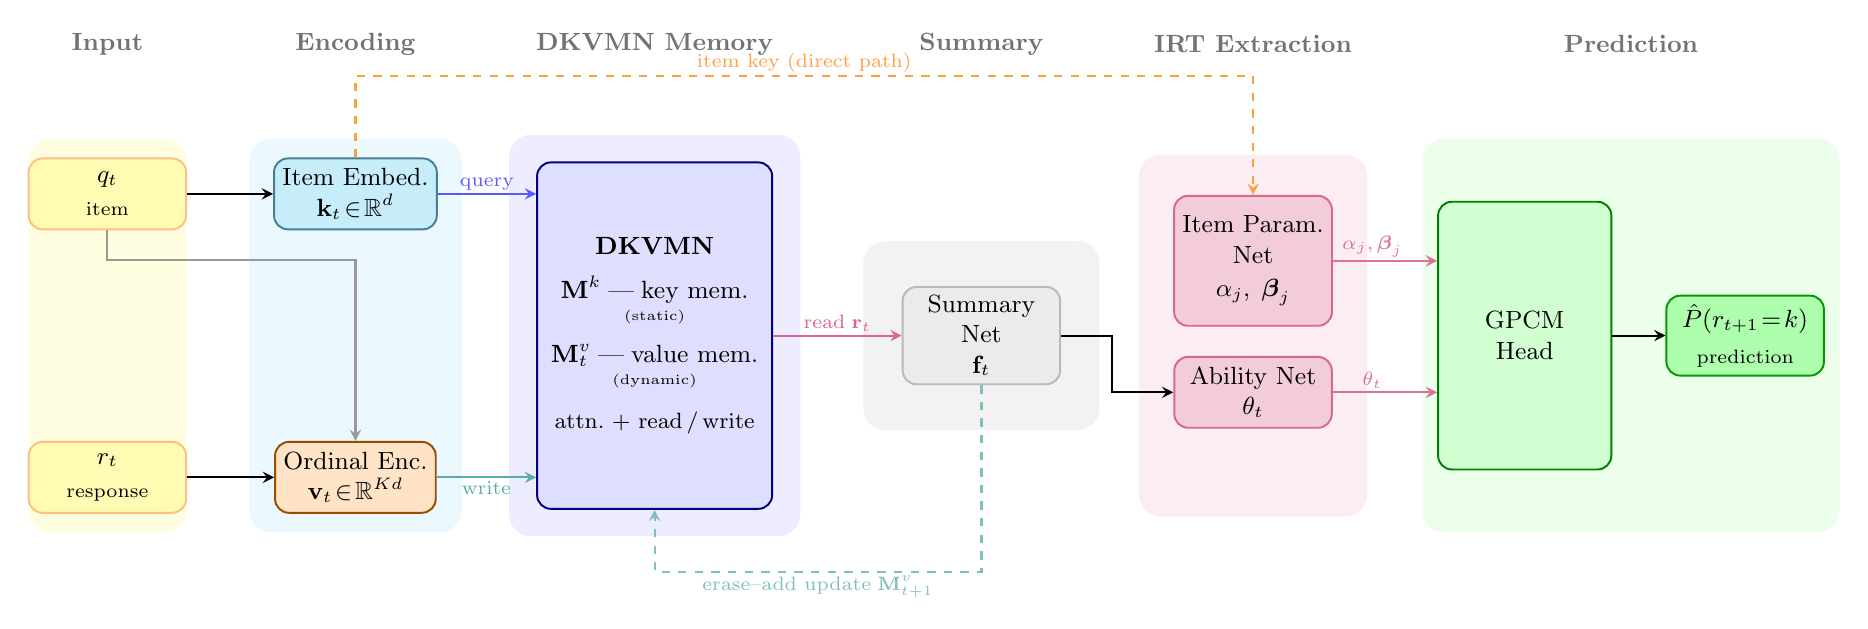
\begin{tikzpicture}[
    >=stealth, line width=0.65pt,
    % --- box styles ---
    box/.style={draw, rounded corners=5pt, minimum width=2.0cm, minimum height=0.90cm,
                align=center, font=\small, inner sep=3pt, line width=0.70pt},
    tallbox/.style={draw, rounded corners=5pt, minimum width=2.2cm,
                    align=center, font=\small, inner sep=5pt, line width=0.70pt},
    % --- arrow styles ---
    arr/.style={->, semithick, line width=0.80pt},
    darr/.style={->, semithick, dashed, line width=0.80pt},
    % --- label style ---
    lbl/.style={font=\scriptsize, inner sep=1pt},
    % --- stage header style ---
    hdr/.style={font=\small\bfseries, text=black!55, inner sep=2pt},
]

%% =====================================================================
%%  COORDINATES (cm)
%%  Cols:  0 = input | 3.3 = encoding | 7.1 = DKVMN | 11.2 = summary
%%         14.6 = IRT | 18.2 = GPCM | 21.4 = output
%%  Rows:  top = 1.80 | mid = 0 | bot = -1.80
%%  Bypass lane: y = 3.30   |   Update loop: y = -3.00
%% =====================================================================

%% ---- BACKGROUND STAGE PANELS (drawn before nodes) ----
\fill[rounded corners=8pt, fill=yellow!12]  (-0.80,-2.50) rectangle ( 1.20, 2.50);
\fill[rounded corners=8pt, fill=cyan!8]     ( 2.00,-2.50) rectangle ( 4.70, 2.50);
\fill[rounded corners=8pt, fill=blue!7]     ( 5.30,-2.55) rectangle ( 9.00, 2.55);
\fill[rounded corners=8pt, fill=gray!10]    ( 9.80,-1.20) rectangle (12.80, 1.20);
\fill[rounded corners=8pt, fill=purple!7]   (13.30,-2.30) rectangle (16.20, 2.30);
\fill[rounded corners=8pt, fill=green!8]    (16.90,-2.50) rectangle (22.20, 2.50);

%% ---- STAGE HEADER LABELS ----
\node[hdr] at ( 0.20, 3.70) {Input};
\node[hdr] at ( 3.35, 3.70) {Encoding};
\node[hdr] at ( 7.15, 3.70) {DKVMN Memory};
\node[hdr] at (11.30, 3.70) {Summary};
\node[hdr] at (14.75, 3.70) {IRT Extraction};
\node[hdr] at (19.55, 3.70) {Prediction};

%% ---- INPUT NODES ----
\node[box, fill=yellow!30, draw=orange!50] (qt) at (0.20,  1.80)
    {$q_t$\\[1pt]{\scriptsize item}};
\node[box, fill=yellow!30, draw=orange!50] (rt) at (0.20, -1.80)
    {$r_t$\\[1pt]{\scriptsize response}};

%% ---- ENCODING NODES ----
\node[box, fill=cyan!22, draw=cyan!55!black] (ke) at (3.35,  1.80)
    {Item Embed.\\$\mathbf{k}_t \!\in\! \mathbb{R}^d$};
\node[box, fill=orange!22, draw=orange!60!black] (oe) at (3.35, -1.80)
    {Ordinal Enc.\\$\mathbf{v}_t \!\in\! \mathbb{R}^{Kd}$};

%% ---- DKVMN MEMORY (tall block with two labelled sub-regions) ----
\node[tallbox, fill=blue!13, draw=blue!50!black, minimum height=4.40cm] (dkvmn) at (7.15, 0)
    {\textbf{DKVMN}\\[5pt]
     $\mathbf{M}^k$\;---\;key mem.\\[-3pt]
     {\tiny (static)}\\[4pt]
     $\mathbf{M}^v_t$\;---\;value mem.\\[-3pt]
     {\tiny (dynamic)}\\[5pt]
     {\footnotesize attn.\ + read\,/\,write}};

%% ---- SUMMARY ----
\node[box, fill=gray!16, draw=gray!55] (summ) at (11.30, 0)
    {Summary\\Net\\$\mathbf{f}_t$};

%% ---- IRT EXTRACTION: two stacked boxes ----
\node[box, fill=purple!20, draw=purple!60, minimum height=1.65cm] (ab) at (14.75,  0.95)
    {Item Param.\\Net\\[1pt]$\alpha_j,\;\boldsymbol{\beta}_j$};
\node[box, fill=purple!20, draw=purple!60] (th) at (14.75, -0.72)
    {Ability Net\\$\theta_t$};

%% ---- GPCM HEAD ----
\node[tallbox, fill=green!18, draw=green!50!black, minimum height=3.40cm] (gpcm) at (18.20, 0)
    {GPCM\\Head};

%% ---- OUTPUT ----
\node[box, fill=green!32, draw=green!60!black] (out) at (21.0, 0)
    {$\hat{P}(r_{t+1}\!=\!k)$\\[2pt]{\scriptsize prediction}};

%% =====================================================================
%%  ARROWS
%% =====================================================================

%% --- Input → Encoding ---
\draw[arr] (qt.east) -- (ke.west);
\draw[arr] (rt.east) -- (oe.west);
%% qt also supplies item identity to ordinal encoding
\draw[arr, black!40] (qt.south) -- ++(0,-0.38) -| (oe.north);

%% --- Encoding → DKVMN ---
%% Key embed → key memory: attention query (blue)
\draw[arr, blue!65] (ke.east)
    -- node[lbl, above, sloped, pos=0.5]{\color{blue!65} query}
    (dkvmn.west |- ke);
%% Ordinal enc → value memory: write (teal)
\draw[arr, teal!65] (oe.east)
    -- node[lbl, below, sloped, pos=0.5]{\color{teal!65} write}
    (dkvmn.west |- oe);

%% --- DKVMN → Summary: attention-weighted read (purple) ---
\draw[arr, purple!60] (dkvmn.east)
    -- node[lbl, above]{\color{purple!60} read\;$\mathbf{r}_t$}
    (summ.west);

%% --- Summary → Ability Net ---
\draw[arr] (summ.east) -- ++(0.65,0) |- (th.west);

%% --- Write-back: Summary → DKVMN (erase--add update, dashed, below) ---
\draw[darr, teal!50] (summ.south)
    -- (11.30, -3.00)
    -- node[lbl, below]{\color{teal!50} erase--add update\;$\mathbf{M}^v_{t+1}$}
    ( 7.15, -3.00)
    -- (dkvmn.south);

%% --- Item key BYPASS → Item Param Net (orange dashed, above) ---
\draw[darr, orange!75] (ke.north)
    -- ( 3.35,  3.30)
    -- node[lbl, above]{\color{orange!75} item key (direct path)}
    (14.75,  3.30)
    -- (ab.north);

%% --- IRT → GPCM ---
\draw[arr, purple!55] (ab.east) -- ++(0.50,0)
    |- node[lbl, above]{\color{purple!55}\scriptsize $\alpha_j,\boldsymbol{\beta}_j$}
    (gpcm.west |- 0, 0.95);
\draw[arr, purple!55] (th.east) -- ++(0.50,0)
    |- node[lbl, above]{\color{purple!55}\scriptsize $\theta_t$}
    (gpcm.west |- 0,-0.72);

%% --- GPCM → Output ---
\draw[arr] (gpcm.east) -- (out.west);

\end{tikzpicture}%
}%
\caption{DEEP-MIRT framework at timestep $t$. Item parameters $(\alpha_j, \boldsymbol{\beta}_j)$ bypass the student state via the item embedding (dashed, top), consistent with the IRT assumption that discrimination and difficulty are student-independent. The GPCM head maps $(\theta_t, \alpha_j, \boldsymbol{\beta}_j)$ to the predicted ordinal distribution $\hat{P}(r_{t+1}=k)$.}
\label{fig:architecture}
\end{figure*}

\subsection{Framework Overview}
\label{sec:framework_overview}

DEEP-MIRT is a modular architecture with two separable concerns. The \emph{backbone} handles the knowledge tracing problem: it encodes item--response interactions, maintains a dynamic memory of the student's evolving knowledge state, and produces a summary vector $\mathbf{f}_t$ representing current student state. The \emph{response head} handles the measurement problem: it maps the backbone's student state $\mathbf{f}_t$ and item identity $\mathbf{k}_t$ to a probability distribution over response categories through a psychometric observation model. Any differentiable function $h(\mathbf{f}_t, \mathbf{k}_t) \to \Delta^{K-1}$ (a distribution over $K$ categories) satisfying this interface is a valid DEEP-MIRT instantiation. The backbone is agnostic to which measurement model governs the head.

This separation is conceptually and practically helpful for tracking learning progressions. The backbone addresses the learning dynamics question of how student ability evolves across a sequence of interactions, naturally handled by sequential neural architectures. The head addresses the measurement question of how current ability maps to the probability of each ordered rubric score, naturally handled by psychometric theory. Coupling them through a clean interface means the two concerns can be improved independently: a better backbone (e.g., Transformer instead of DKVMN) improves temporal modeling without changing the interpretable parameterization; a different head (e.g., GRM instead of GPCM) changes the measurement assumptions without retraining the backbone.

In this paper we instantiate the head as the \textbf{Generalized Partial Credit Model} (GPCM, Section~\ref{sec:polytomous_irt}). We chose GPCM over the other major polytomous families for three reasons: (1) it is an adjacent-category model, which is the natural match for rubric scoring where a student progresses sequentially through performance levels; (2) it produces a discrimination parameter $\alpha_j$ and ordered step difficulty thresholds $\boldsymbol{\beta}_j$ that correspond directly to rubric design decisions and can be inspected by assessment practitioners; (3) its monotone threshold constraint admits a clean differentiable parameterization (Section~\ref{sec:gpcm_head}). A cumulative model such as the Graded Response Model~\citep{samejima_estimation_1969} would be a natural alternative for tasks where each scoring threshold represents an independent decision (e.g., analytic rubrics with independent sub-scores); a Nominal Response Model~\citep{bock_estimating_1972} would apply when response categories are unordered (e.g., multiple-choice distractors encoding different misconceptions). We treat these as directions for future instantiation.

The backbone processes inputs through four sequential stages as shown in Figure~\ref{fig:architecture}: ordinal interaction encoding, DKVMN memory update, summary compression, and IRT-based parameter extraction. An ordinal-aware training objective supervises all stages jointly. The following subsections formalize each component.

\subsection{Problem Formulation}
Let $r_t \in \{0,1,\ldots,K-1\}$ denote an observed response with $K$ \emph{ordered} categories (e.g., rubric levels / partial credit),
and let $q_t \in \{0,1\}^Q$ be a one-hot indicator of the exercised question/item, where $Q$ is the number of unique items.
An interaction is $x_t=(q_t,r_t)$ and the observed history up to time $t$ is
$\mathcal{X}_t=\{(q_1,r_1),\ldots,(q_t,r_t)\}$.
We study \emph{ordinal} (polytomous) knowledge tracing as predicting the full distribution
\begin{equation}
    P(r_{t+1}=k \mid q_{t+1}, \mathcal{X}_t), \quad k \in \{0,\ldots,K-1\}.
\end{equation}

\subsection{Ordinal-Aware Interaction Representation}
\paragraph{Linear Decay Encoding}
We encode an ordinal response $r_t$ with a ``triangular'' kernel over ordered categories.
Define a length-$K$ ordinal code $\mathbf{s}_t \in \mathbb{R}^{K}$ by
\begin{equation}\label{eqn:linear_embed}
    \begin{split}
    s_t^{(k)}&=\max\!\left(0,1-\frac{|k-r_t|}{K-1}\right),\quad 0\le k\le K-1,\\
    \mathbf{s}_t&=[s_t^{(0)};\ldots;s_t^{(K-1)}].
    \end{split}
\end{equation}
For example, with a $K=4$ rubric and a response of $r_t = 2$ (``correct approach with errors''), the ordinal code is $\mathbf{s}_t = [0.33,\; 0.67,\; 1.0,\; 0.67]$, which spreads activation to neighboring categories while peaking at the observed level. This encoding preserves the ordinal structure: a response of 2 is represented as more similar to responses 1 and 3 than to response 0, reflecting the educational intuition that partial credit is closer to full credit than to no credit.

We then bind the ordinal code to the item indicator via a Kronecker product (equivalently, a block one-hot expansion):
\begin{equation}
    \mathbf{x}_t = q_t \otimes \mathbf{s}_t \in \mathbb{R}^{KQ}.
\end{equation}
This reduces to the standard binary interaction encoding when $K=2$ (consistent with \citet{zhang_dynamic_2017}).
While this encoding is effective for moderately sized item banks, the $\mathcal{O}(KQ)$ dimensionality becomes a practical constraint for large $Q$; we address this in the following subsection.

\paragraph{Scalable Value Encoding for Large Item Banks}
Large-scale educational platforms maintain extensively large item banks with various grade levels. The triangular Kronecker encoding in \eqref{eqn:linear_embed} yields an interaction vector of dimension $KQ$, which grows linearly with item bank size. The subsequent value projection $\mathbf{v}_t = B^{\top}\mathbf{x}_t \in \mathbb{R}^{d_v}$ therefore requires a $KQ \times d_v$ weight matrix; at $Q = 5{,}000$ and $K = 5$, this amounts to 1.6M parameters and a per-batch intermediate tensor of size $\mathrm{batch} \times S \times 25{,}000$, placing substantial memory pressure on GPU-constrained deployment environments.

We propose \textbf{Static Item Embedding} (SIE), an alternative value encoding that decouples item identity from response pattern via two independent additive branches:
\begin{equation}\label{eqn:sie}
    \mathbf{v}_t = W_{\mathrm{item}}\,\mathbf{u}_{q_t} + W_{\mathrm{resp}}\,\mathbf{s}_t + \mathbf{b}_{\mathrm{resp}} \in \mathbb{R}^{d_v},
\end{equation}
where $\mathbf{u}_{q_t} \in \mathbb{R}^{H}$ is a \emph{frozen} (non-trainable) unit-norm random vector assigned to item $q_t$ at initialization, $\mathbf{s}_t \in \mathbb{R}^K$ is the triangular ordinal code from \eqref{eqn:linear_embed}, and $W_{\mathrm{item}} \in \mathbb{R}^{d_v \times H}$ and $W_{\mathrm{resp}} \in \mathbb{R}^{d_v \times K}$ are learned projections shared across all items.

The factored structure in \eqref{eqn:sie} separates two gradient channels: $W_{\mathrm{item}}$ is updated by item-identity signals, while $W_{\mathrm{resp}}$ is updated by response-pattern signals. Because item vectors are frozen, items cannot collapse to similar representations during training, a failure mode of learned separable embeddings at large $Q$ (cf.\ Section~\ref{sec:ablation_sensitivity}). For two independent uniformly random unit vectors in $\mathbb{R}^H$, the expected squared inner product is $1/H$ \citep{dasgupta_elementary_2003}, so pairwise interference concentrates around zero as $H$ grows; cross-item gradient crosstalk in $W_{\mathrm{item}}$ therefore decays with $H$ independently of $Q$, making SIE well-suited for large item banks.

The frozen dimension $H$ is set as the smallest power of two no less than $\max(128, \lfloor Q/2 \rfloor)$, clamped to $[128, 1024]$.\footnote{Concretely, $H = 128$ for $Q \le 256$, $H = 256$ for $Q \approx 500$, $H = 512$ for $Q \approx 1{,}000$, and $H = 1{,}024$ for $Q \ge 2{,}000$.} This schedule ensures near-orthogonality scales with item bank size while keeping the projection dimension bounded, in contrast to the $\mathcal{O}(KQ)$ complexity of the full Kronecker encoding.

\subsection{Dynamic Key-Value Memory Network}
We adopt the Dynamic Key-Value Memory Network (DKVMN) as the sequential backbone.
Let $\mathbf{k}_t = A^{\top} q_t \in \mathbb{R}^{d_k}$ be a key embedding for the current item and
$\mathbf{v}_t \in \mathbb{R}^{d_v}$ be a value embedding for the interaction, obtained via the Kronecker projection $\mathbf{v}_t = B^{\top}\mathbf{x}_t$ (ordinal-aware encoding) or the Static Item Embedding in \eqref{eqn:sie} (scalable encoding).
The model maintains a static key memory $\mathbf{M}^k \in \mathbb{R}^{N \times d_k}$ and
a dynamic value memory $\mathbf{M}^v_t \in \mathbb{R}^{N \times d_v}$.
Educationally, the key memory represents latent skill areas or knowledge components, the value memory tracks the student's evolving mastery of each area, and the attention weights $\mathbf{w}_t$ (below) indicate which skill areas a given item exercises. The summary vector $\mathbf{f}_t$ aggregates the student's current mastery state relevant to the item at hand.

Specifically, the key query is first projected via a learned transform, and attention weights over memory slots are computed as
\begin{equation}
    \tilde{\mathbf{k}}_t=\tanh(W_{\mathrm{attn}}\mathbf{k}_t),\qquad
    \mathbf{w}_t=\mathrm{softmax}(\mathbf{M}^k \tilde{\mathbf{k}}_t)\in\mathbb{R}^{N},\qquad
    w_t(i)=[\mathbf{w}_t]_i,
\end{equation}
and the read vector is
\begin{equation}
    \mathbf{r}_t=\sum_{i=1}^{N} w_t(i)\,\mathbf{M}_t^v(i)\in\mathbb{R}^{d_v}.
\end{equation}
We fuse item context and retrieved state into a summary vector
\begin{equation}\label{eqn:summary_vec}
    \mathbf{f}_t=\tanh\!\left(W_{\mathbf{f}}[\mathbf{r}_t;\mathbf{k}_t]+b_{\mathbf{f}}\right),
\end{equation}
which is then used by the response head to predict $r_{t+1}$.

Following memory-augmented neural networks, the value memory is updated via erase-add operations:
\begin{align}
\mathbf{e}_t&=\sigma(W_{\mathbf{e}}\mathbf{v}_t+b_{\mathbf{e}}),\label{eqn:erase_vec}\\
\mathbf{a}_t&=\tanh(W_{\mathbf{a}}\mathbf{v}_t+b_{\mathbf{a}}),\label{eqn:add_vec}\\
\mathbf{M}_{t+1}^v(i)&=\mathbf{M}_{t}^v(i)\bigl[1-w_t(i)\mathbf{e}_t\bigr]+w_t(i)\mathbf{a}_t.\label{eqn:value_memory_update}
\end{align}

\subsection{DEEP-GPCM: an Ordinal IRT Head}
\label{sec:gpcm_head}
Instead of the binary readout (e.g., $\sigma(W_p^{\top}\mathbf{f}_t+b_p)$), we use a Generalized Partial Credit Model (GPCM) head
to obtain category probabilities for ordered responses.
Let $j$ denote the item exercised at time $t$ (i.e., $[q_t]_j=1$).
We compute a time-varying ability proxy $\theta_t$ and item-specific parameters (thresholds and discrimination) as
\begin{align}
    \theta_t &= W_{\theta}\mathbf{f}_t+b_{\theta}, \label{eqn:ability_net}\\
    \beta_{j,0} &= W_{\beta}\mathbf{k}_t+b_{\beta}, \label{eqn:b_0}\\
    \beta_{j,k} &= \beta_{j,k-1}+\mathrm{softplus}(W_{g[k]}\mathbf{k}_t+b_{g[k]}),\quad 1\le k\le K-2, \label{eqn:b_k}\\
    \alpha_{j} &= \exp\!\left(W_{\alpha}\mathbf{k}_t+b_{\alpha}\right). \label{eqn:diff_net}
\end{align}
The construction in \eqref{eqn:b_k} enforces $\beta_{j,0}<\beta_{j,1}<\cdots<\beta_{j,K-2}$ by adding strictly positive increments (via softplus) to each preceding threshold. This monotonicity guarantee has direct educational meaning: achieving rubric level $k{+}1$ always requires higher ability than achieving level $k$, respecting the ordering that a rubric designer intended. Without this constraint, the model could learn disordered thresholds where some rubric levels are never the most probable response at any ability level, a well-documented problem in educational measurement that signals a poorly functioning item \citep{wilson_constructing_2005}.

Because discrimination is an item-intrinsic property in the GPCM, $\alpha_j$ is derived solely from the item key $\mathbf{k}_t$, deliberately excluding the student-state summary $\mathbf{f}_t$. This separation ensures that the estimated discrimination reflects the item's inherent capacity to differentiate ability levels, independently of which student is currently being modelled — consistent with the IRT assumption that item parameters are population-invariant \citep{hambleton_item_1985}. Item-level discrimination is recovered by averaging per-timestep estimates across all encounters with a given item \citep{meulders_person-by-item_2004}. The exponential activation ensures $\alpha_j > 0$.

Given $(\theta_t,\alpha_j,\{\beta_{j,k}\}_{k=0}^{K-2})$, the GPCM category probability is
\begin{equation}\label{eqn:gpcm_prob}
    p_{t,k}=
    \frac{\exp\!\left(\sum_{i=0}^{k-1}\alpha_j(\theta_t-\beta_{j,i})\right)}
         {\sum_{c=0}^{K-1}\exp\!\left(\sum_{i=0}^{c-1}\alpha_j(\theta_t-\beta_{j,i})\right)}.
\end{equation}
At each timestep, the model evaluates this standard GPCM formulation (cf.\ Section~\ref{sec:polytomous_irt}) using the \emph{dynamically estimated} student ability $\theta_t$ and item parameters $\alpha_j, \boldsymbol{\beta}_j$. Unlike classical GPCM estimation where ability is static, here $\theta_t$ evolves as new interactions are observed, enabling the model to track learning over time while retaining the interpretable measurement structure of polytomous IRT.

We predict $\hat{r}_{t+1}=\arg\max_k p_{t,k}$, and optimize the combined ordinal loss in \eqref{eqn:combined_loss} over the observed responses.

\subsection{Training Objective for Ordinal Data}
Because the GPCM defines category probabilities via \eqref{eqn:gpcm_prob} rather than cumulative links,
we optimize a weighted categorical objective with an ordinal distance penalty to mitigate class imbalance \citep{gutierrez_ordinal_2016}.
The loss combines two complementary components:
\begin{equation}\label{eqn:combined_loss}
\mathcal{L}=\lambda_{\mathrm{focal}}\mathcal{L}_{\mathrm{focal}}+\lambda_{\mathrm{WOL}}\mathcal{L}_{\mathrm{WOL}},
\end{equation}
where $\mathcal{L}_{\mathrm{focal}}$ is the focal loss \citep{lin_focal_2020}, which down-weights well-classified examples and focuses training on ambiguous responses near category boundaries.
The weighted ordinal loss $\mathcal{L}_{\mathrm{WOL}}$ is
\begin{equation}\label{eqn:wol_loss}
    \mathcal{L}_{\mathrm{WOL}}
    =\frac{1}{n}\sum_{i=1}^{n}\Bigl[(1+\gamma|y_i-\hat{y}_i|)\cdot w_{y_i}\cdot(-\log \hat{p}_{i,y_i})\Bigr],
\end{equation}
where $y_i$ is the true category, $\hat{p}_{i,y_i}$ is the predicted probability under \eqref{eqn:gpcm_prob},
$\hat{y}_i=\arg\max_k \hat{p}_{i,k}$ is the predicted label, and $\gamma$ controls the ordinal distance penalty.
To balance classes, with $c_k$ the sample count of class $k$, we set $w_k=\sqrt{\frac{n}{K\cdot c_k}}$, where $n$ is the number of valid tokens in the batch.

\section{Experiments}

% \subsection{Experimental Settings}

% Unless otherwise stated, all results below use \textbf{single-trait} instantiations of DEEP-MIRT; multidimensional extensions are part of future work.

\subsubsection{Datasets}
\paragraph{Synthetic-Ordinal.}
To the best of our knowledge, there are no standardized public benchmarks for ordinal knowledge tracing. We therefore generate a synthetic dataset using an IRT-GPCM data generating process following established psychometric principles. This design provides controlled polytomous supervision $r_t\in\{0,\ldots,K-1\}$ and enables parameter recovery analysis with known ground truth.

We simulate $5{,}000$ students interacting with questions drawn from a pool of $Q=200$ questions in random order. Each interaction sequence has variable length in $[50,200]$. Students and questions are configured with \emph{static} GPCM parameters following assumed priors:
\begin{itemize}
    \item \textit{Student ability:} $\theta\sim\mathcal{N}(0,1)$,
    \item \textit{Item discrimination:} $\alpha\sim \mathrm{LogNormal}(0,0.3)$,
    \item \textit{Item thresholds:} $K{-}1$ values drawn independently from $\mathcal{N}(0,1)$ and sorted to obtain $\beta_0<\cdots<\beta_{K-2}$.
\end{itemize}
We generate four datasets with $K\in\{2,3,4,5\}$ to test extensibility across category resolutions. Each dataset is split 80/20 for training/testing; a validation split is held out from training for early stopping and hyperparameter tuning.

\paragraph{Proxy-Ordinality}
To test our model on real educational logs, we derive ordinal labels from attempt counts in ASSISTments-style data (e.g., 1 attempt $=$ mastery, 2--3 $=$ partial, 4+ $=$ struggle). Results and evaluation details are described in Section~\ref{sec:proxy_results}.

\paragraph{Binary Compatibility}
After validating the PKT instantiations on Synthetic-Ordinal, we confirm compatibility with binary KT. Due to implementation differences in batch handling and sequence-to-question lookup, we select two datasets:
\begin{itemize}
    \item \textbf{ASSIST2015}\footnote{https://sites.google.com/site/assistmentsdata/datasets/2015-assistments-skill-builder-data}: 19,840 students and 100 KCs/questions.
    \item \textbf{Synthetic-5}\footnote{\url{https://github.com/chrispiech/DeepKnowledgeTracing/tree/master/data/synthetic}}: \citep{piech_deep_2015} simulated 4,000 students' responses with probability $p(r)=c+\frac{1}{1+\exp(-(\theta-\beta))}$ where $c=0.25$ models question guessing. Each student is administered 50 questions in sequential order.
\end{itemize}

\subsubsection{Models and Baselines}
We compare DEEP-GPCM against three baselines that progressively relax psychometric and ordinal structure, each isolating a different design question:
\begin{itemize}
    \item \textbf{DKVMN + Softmax}: DKVMN backbone with a $K$-way softmax head trained with categorical cross-entropy. No ordinal structure, no IRT constraints. Tests whether psychometric parameterization provides gains over a purely neural polytomous baseline.
    \item \textbf{DKVMN + Ordinal}: DKVMN backbone with a linear output head trained using the weighted ordinal loss \eqref{eqn:wol_loss}. Introduces ordinal awareness without IRT parameterization, isolating the contribution of the GPCM structure over simpler ordinal objectives.
    \item \textbf{Static GPCM}: Standard GPCM fit from interaction data with student ability held fixed across items. No sequential dynamics. Represents the psychometric status quo and quantifies what sequential modeling adds beyond classical IRT estimation.
    \item \textbf{DEEP-GPCM (ours)}: DKVMN backbone with GPCM head and combined ordinal loss \eqref{eqn:combined_loss}. Uses SIE encoding by default; the choice of encoding strategy is ablated in Section~\ref{sec:ablation_sensitivity}.
\end{itemize}
For dichotomous KT ($K=2$), we additionally compare against \textbf{DKT} \citep{piech_deep_2015} and \textbf{DKVMN} \citep{zhang_dynamic_2017} as established binary baselines.

\subsubsection{Prediction Mapping}
For $K=2$, predicted probabilities are converted to labels with a threshold of 0.5 following \citet{zhang_dynamic_2017}. For $K>2$, we use $\hat{y}_t=\arg\max_k \hat{p}_{t,k}$ to map categorical probabilities to prediction labels.

\subsubsection{Training Setup}
We use the combined loss in \eqref{eqn:combined_loss} to handle class imbalance and ordinal agreement, with tunable weights $\lambda_{*}$.

We set $d_k=64$ and $d_v=128$ for key/value embedding dimensions and configure $N=50$ memory slots for both memory matrices.

All models are trained with batch size 64 using Adam with learning rate $10^{-3}$, reduced on performance plateau as per \citet{mukherjee_simple_2019} for late-epoch stability. We apply dropout 0.05 and early stopping if validation loss does not improve for 10 epochs. Models are implemented in PyTorch and trained on an RTX 4060 Laptop GPU.

\subsubsection{Evaluation Metrics}
We use the following metrics:
\begin{itemize}
    \item \textbf{Categorical Accuracy (ACC)}: percentage of exact matches between predicted category and ground truth. While straightforward, ACC does not distinguish near-misses from far-misses and is therefore insufficient as a sole ordinal metric.
    \item \textbf{Quadratic Weighted Kappa (QWK)} \citep{cohen_weighted_1968}: our primary metric for ordinal tasks. QWK applies a quadratic penalty proportional to the squared distance between predicted and true categories, making it the standard agreement measure in automated essay scoring and rubric evaluation. A QWK of 0.0 indicates chance-level agreement; 1.0 indicates perfect agreement.
    \item \textbf{Kendall's Tau ($\boldsymbol{\tau}$)}: measures rank-order agreement between predicted and true response sequences, penalizing all inversions equally regardless of distance.
    \item \textbf{Area Under the ROC Curve (AUC)}: used for the binary case ($K=2$) to maintain comparability with prior KT literature.
\end{itemize}

\subsubsection{IRT Analysis Setup}
For parameter recovery analysis on Synthetic-Ordinal, we use:
\begin{itemize}
    \item $\boldsymbol{\theta}$ \textbf{Aggregation}: we take the mean ability estimate $\bar{\theta} = \frac{1}{T}\sum_{t=1}^{T}\theta_t$ across all timesteps for each student, averaging out sequence-position noise while exploiting the full interaction history.
    \item $\boldsymbol{\alpha}, \boldsymbol{\beta}$ \textbf{Aggregation}: because questions appear with variable frequency due to random sequencing, we aggregate item parameters based on occurrences and use the sample mean for recovery analysis.
\end{itemize}
We normalize learned parameters and true parameters using the priors used to generate each dataset. Specifically, both $\theta$ and $\beta$ use z-score normalization. $\alpha$ is log-transformed and standardized with log-mean and log-standard deviation; we then rescale by 0.3 before the final exponential projection to match the generating scale.

\subsection{Results}

\subsubsection{Ordinal Prediction on Synthetic-Ordinal (RQ1)}
Table~\ref{tab:comp_results} reports prediction performance on Synthetic-Ordinal for $K\in\{2,3,4,5\}$, addressing \textbf{RQ1}. DEEP-GPCM results are complete; baseline results are pending implementation (see note below). For DEEP-GPCM, ordinal agreement improves with category resolution: QWK rises from 0.618 at $K=3$ to 0.758 at $K=5$, and Kendall's $\tau$ from 0.567 to 0.655, indicating that the GPCM head effectively exploits the finer ordinal structure available in higher-$K$ rubrics.

\begin{table*}[htb!]
\centering
\caption{Synthetic-Ordinal results across $K\in\{2,3,4,5\}$ on Synthetic-Ordinal ($Q=200$). Dashes indicate pending experiments. Best completed results in bold.}
\label{tab:comp_results}
\begin{subtable}[t]{0.49\textwidth}
\centering
\caption{$K=2$ (Binary)}
\small
\setlength{\tabcolsep}{3pt}
\begin{tabular}{lccc}
\toprule
\textbf{Model} & \textbf{Acc(\%)} & \textbf{AUC} & $\boldsymbol{\tau}$ \\
\midrule
DKT & --- & --- & --- \\
DKVMN & --- & --- & --- \\
\midrule
DEEP-GPCM & \textbf{71.4} & \textbf{0.795} & \textbf{0.434} \\
\bottomrule
\end{tabular}
\end{subtable}
\hfill
\begin{subtable}[t]{0.49\textwidth}
\centering
\caption{$K=3$}
\small
\setlength{\tabcolsep}{3pt}
\begin{tabular}{lccc}
\toprule
\textbf{Model} & \textbf{Acc(\%)} & \textbf{QWK} & $\boldsymbol{\tau}$ \\
\midrule
DKVMN + Softmax & --- & --- & --- \\
DKVMN + Ordinal & --- & --- & --- \\
Static GPCM & --- & --- & --- \\
\midrule
DEEP-GPCM & \textbf{60.7} & \textbf{0.618} & \textbf{0.567} \\
\bottomrule
\end{tabular}
\end{subtable}

\vspace{0.5em}
\begin{subtable}[t]{0.49\textwidth}
\centering
\caption{$K=4$}
\small
\setlength{\tabcolsep}{3pt}
\begin{tabular}{lccc}
\toprule
\textbf{Model} & \textbf{Acc(\%)} & \textbf{QWK} & $\boldsymbol{\tau}$ \\
\midrule
DKVMN + Softmax & --- & --- & --- \\
DKVMN + Ordinal & --- & --- & --- \\
Static GPCM & --- & --- & --- \\
\midrule
DEEP-GPCM & \textbf{53.7} & \textbf{0.710} & \textbf{0.627} \\
\bottomrule
\end{tabular}
\end{subtable}
\hfill
\begin{subtable}[t]{0.49\textwidth}
\centering
\caption{$K=5$}
\small
\setlength{\tabcolsep}{3pt}
\begin{tabular}{lccc}
\toprule
\textbf{Model} & \textbf{Acc(\%)} & \textbf{QWK} & $\boldsymbol{\tau}$ \\
\midrule
DKVMN + Softmax & --- & --- & --- \\
DKVMN + Ordinal & --- & --- & --- \\
Static GPCM & --- & --- & --- \\
\midrule
DEEP-GPCM & \textbf{48.7} & \textbf{0.758} & \textbf{0.655} \\
\bottomrule
\end{tabular}
\end{subtable}
\end{table*}

\begin{pendingbox}[Pending: baseline experiments for RQ1]
Three baselines remain to be implemented and evaluated on Synthetic-Ordinal.
\begin{itemize}
  \item \textbf{DKVMN + Softmax}: Expected to achieve competitive accuracy but lower QWK and $\tau$ than DEEP-GPCM, since treating rubric levels as unordered categories ignores ordinal distance in prediction.
  \item \textbf{DKVMN + Ordinal}: Expected to close part of the QWK gap over Softmax by penalising distant misclassifications. Whether it matches DEEP-GPCM will test whether the GPCM parameterization adds value beyond the ordinal loss alone.
  \item \textbf{Static GPCM}: Expected to lag dynamic models substantially, particularly on longer sequences, as it cannot adapt ability estimates across interactions. Recovery of $\alpha$ and $\beta$ may be comparatively clean, providing a useful psychometric reference point.
\end{itemize}
Implementation note: DKVMN + Softmax and DKVMN + Ordinal share the backbone and differ only in the output head and loss; Static GPCM requires a standard marginal maximum likelihood fitting routine (e.g., EM with normal-ogive approximation).
\end{pendingbox}

\subsubsection{Binary Compatibility on Standard KT Benchmarks}
An important practical requirement is that a polytomous KT model should not sacrifice performance when deployed on standard binary data, since many existing item banks and datasets use dichotomous scoring, and a useful framework must handle both formats without architectural modification. We evaluate backward compatibility by instantiating DEEP-MIRT with $K=2$ and testing on ASSIST2015 and Synthetic-5. Results are reported in Table~\ref{tab:combined_perf}. DEEP-GPCM achieves competitive performance compared to DKT and DKVMN despite substituting the binary readout with a GPCM head, confirming that the GPCM head gracefully degenerates to a standard logistic model when $K=2$.

\begin{table}[htb!]
\centering
\caption{Test results on selected metrics for ASSIST2015 and Synthetic-5. The best results for each metric are highlighted in bold.}
\label{tab:combined_perf}
\begin{tabular}{lcccc}
\toprule
\textbf{Model} & \multicolumn{2}{c}{\textbf{ASSIST2015}} & \multicolumn{2}{c}{\textbf{Synthetic-5}} \\
\cmidrule(lr){2-3} \cmidrule(lr){4-5}
& \textbf{ACC} & \textbf{AUC} & \textbf{ACC} & \textbf{AUC} \\
\midrule
DKT & 75.2\% & 0.727 & \textbf{75.2}\% & 0.817 \\
DKVMN & 75.1\% & \textbf{0.729} & 75.1\% & \textbf{0.827} \\
DEEP-GPCM & \textbf{75.4\%} & 0.723 & 74.7\% & 0.824 \\
\bottomrule
\end{tabular}
\end{table}

\subsubsection{IRT Parameter Recovery and Stability (RQ2)}
\label{sec:irt_analysis}
A key advantage of DEEP-MIRT is that it produces psychometrically meaningful parameters alongside predictions, addressing \textbf{RQ2}. Student ability ($\theta$) and step difficulty thresholds ($\beta_k$) show strong alignment with ground-truth IRT parameters, because both are tied to the DKVMN memory summary that accumulates interaction history. Discrimination recovery varies significantly with encoding choice and is analysed in the Ablation section below. A systematic compression of learned thresholds toward the centre is observed: the model tends to place step difficulties closer together than their true values, a limitation for applications requiring precise threshold estimates such as cut-score setting.

Figure~\ref{fig:recovery} shows parameter recovery for the SIE model trained on the \texttt{large\_q5000} dataset ($Q=5{,}000$, $K=5$). Step difficulty thresholds ($\beta_k$) are recovered with high fidelity across all four steps ($r_{\beta} = 0.88$--$0.93$, mean $r_{\beta} = 0.90$), confirming that the DKVMN memory accumulates sufficient item-specific information to place thresholds accurately. Discrimination recovery is moderate ($r_\alpha \approx 0.65$), consistent with the known difficulty of identifying item-level discrimination from observational sequences; items with low ground-truth discrimination ($\alpha_j < 0.5$) are recovered with lower correlation, consistent with classical IRT estimation theory. Student ability recovery is low ($r_\theta = 0.21$) on this static-$\theta$ synthetic dataset, which reflects a measurement artefact rather than a model limitation: because each student's true $\theta$ is fixed at generation time, the model's time-varying estimate $\hat{\theta}_t$ reflects posterior convergence rather than a ground-truth signal that changes across interactions. Recovery of $\theta$ on dynamic-$\theta$ data is a planned experiment (see Section~\ref{sec:trajectories}).

\begin{figure}[htb!]
\centering
\includegraphics[width=\linewidth]{kt-gpcm/outputs/large_q5000_static/recovery_figure.png}
\caption{IRT parameter recovery for DEEP-GPCM (SIE encoding, $Q=5{,}000$, $K=5$, $N=1{,}000$ students). \emph{Top left}: kernel density of true vs.\ mean estimated student ability $\hat{\theta}$ (z-scored to $\mathcal{N}(0,1)$); the low Pearson $r=0.21$ is a data artefact — each student's true $\theta$ is constant at generation time, so the model's time-varying estimate $\hat{\theta}_t$ reflects posterior convergence rather than a changing signal. \emph{Top right}: discrimination recovery in log-linked space ($r_\alpha=0.67$), showing the expected moderate correlation for item-level discrimination from observational sequences. \emph{Bottom row}: step-difficulty recovery for each of the four GPCM thresholds $\beta_1$--$\beta_4$ individually (z-scored per threshold); $r_{\beta_1}=0.88$, $r_{\beta_2}=0.93$, $r_{\beta_3}=0.92$, $r_{\beta_4}=0.87$ (mean $r=0.90$), confirming strong item calibration across all difficulty levels.}
\label{fig:recovery}
\end{figure}

\begin{pendingbox}[Pending: recovery for $K\in\{2,3\}$, split-half reliability, and dynamic-$\theta$ data]
Full recovery results for other $K$ values and the Static GPCM baseline are pending. Split-half reliability will divide students into two random halves and correlate $\hat{\alpha}_j$, $\hat{\beta}_{j,k}$ across halves; correlations exceeding $r=0.90$ constitute strong evidence of measurement stability \citep{embretson_irt_2000}. Recovery of $\theta$ will be re-evaluated once the dynamic-$\theta$ data generator is available.
\end{pendingbox}

\subsubsection{Learner State Dynamics (RQ3)}
\label{sec:trajectories}
A distinctive property of DEEP-GPCM is that the DKVMN memory produces a temporally-indexed ability estimate $\theta_t$ at each interaction step, rather than a single post-hoc score. This enables assessment of whether the inferred student state exhibits psychologically plausible learning dynamics, directly addressing \textbf{RQ3}. Because DKVMN + Softmax produces a latent summary vector rather than a scalar ability, we construct a comparable learner state proxy from its predictions as the expected score $\hat{s}_t = \sum_{k=0}^{K-1} k \cdot \hat{p}_{t,k}$, which lies on the same $[0, K-1]$ scale as the ordinal response and provides the most interpretable single-number summary of the model's categorical forecast. Comparing $\theta_t$ from DEEP-GPCM against $\hat{s}_t$ from DKVMN + Softmax allows us to assess whether psychometric grounding yields qualitatively different and more interpretable portraits of student learning.

We examine trajectories for three learner archetypes on held-out synthetic students with known ground-truth $\theta$: (i) a \emph{high-ability} learner whose true $\theta$ places them consistently in the upper tail of the ability distribution; (ii) a \emph{struggling} learner with low true $\theta$ who produces predominantly zero or near-zero category responses throughout the sequence; and (iii) a \emph{growth} learner whose response pattern shows systematic improvement over the sequence, enabling examination of whether $\theta_t$ rises in accordance with the improving response record. For each archetype, trajectory plots show $\theta_t$ (DEEP-GPCM) and $\hat{s}_t$ (DKVMN + Softmax) side by side across interaction steps, with ground-truth $\theta$ displayed as a horizontal reference line for the synthetic condition. Qualitative inspection of $\theta_t$ on completed runs already confirms that students with higher ground-truth $\theta$ converge to higher ability estimates, and that ability trajectories show monotone growth for students with consistently improving responses, consistent with theoretical expectations.

\begin{figure}[htb!]
\centering
\includegraphics[width=\linewidth]{kt-gpcm/outputs/large_q5000_static/trajectory_plots/learner_trajectories.png}
\caption{Learner state trajectories for four student archetypes from the \texttt{large\_q5000} dataset ($K=5$, SIE encoding, $D=1$). Blue: DEEP-GPCM expected score $\hat{s}_t = \sum_k k\,\hat{p}_{t,k}$. Orange dashed: DEEP-GPCM $\theta_t$ rescaled linearly to $[0, K{-}1]$. Black dashed: ground-truth $E[r \mid \theta^*, \alpha_\text{ref}, \beta_\text{ref}]$ for a reference item with $\beta_0 \approx 0$ and $\alpha = 1.13$. High- and low-ability students converge within roughly 50--100 interactions; mid-ability and ambiguous students show the expected residual variance around the midpoint. The close tracking between the blue and orange curves confirms that $\theta_t$ is consistent with the model's predicted category distribution. All curves smoothed with a 9-step rolling mean.}
\label{fig:trajectories}
\end{figure}

\begin{pendingbox}[Pending: DKVMN + Softmax comparison for RQ3]
Figure~\ref{fig:trajectories} currently shows DEEP-GPCM trajectories only. Once the DKVMN + Softmax baseline is trained, its $\hat{s}_t$ curve will be overlaid on each panel, allowing direct comparison of convergence speed, trajectory smoothness, and alignment with ground truth. A quantitative monotonicity summary (proportion of students with net positive $\theta_t$ change in high-ability conditions, split by ability quartile) will accompany the updated figure.
\end{pendingbox}

\subsubsection{Scalable Item Encoding (RQ4)}
\label{sec:scalability}
We address \textbf{RQ4} by comparing three item encoding strategies on a large-scale dataset ($Q=5{,}000$, $K=5$, sequences of length $[400,600]$, 1{,}000 students), where the cost of dense encoding becomes practically significant. Table~\ref{tab:recovery} reports QWK and IRT parameter recovery for LinearDecay, Separable, and SIE encodings. All models use $d_k=d_v=64$ and $N=50$ memory slots; batch size 16 (reduced from 64 to accommodate LinearDecay's $\mathrm{batch}\times S\times KQ$ input tensor). All three complete each epoch in 127--129 s, confirming that wall-clock throughput is governed by the DKVMN memory loop and not by the encoding stage. SIE achieves the best QWK (0.778) and the strongest discrimination recovery ($r_\alpha=0.654$) at only 408K parameters — approximately one-fifth of LinearDecay's 1.9M — establishing SIE as the preferred encoding when both prediction quality and psychometric recovery matter at scale.

\begin{table}[htb!]
\centering
\caption{Item encoding comparison at $Q=5{,}000$, $K=5$, sequence length $\sim\!500$. $r_\alpha$ and $r_\beta$ are Pearson correlations with ground-truth IRT parameters ($r_\beta$ is the pooled correlation across all $K{-}1$ thresholds; Figure~\ref{fig:recovery} reports per-step values for SIE). $r_\theta$ values for LinearDecay and Separable are pending.}
\label{tab:recovery}
\small
\setlength{\tabcolsep}{4pt}
\begin{tabular}{lrrccc}
\toprule
\textbf{Encoding} & \textbf{Params} & \textbf{QWK} & $r_\theta$ & $r_\alpha$ & $r_\beta$ \\
\midrule
LinearDecay & 1{,}943K & 0.762 & --- & 0.022 & 0.906 \\
Separable   &   667K  & 0.773 & --- & 0.246 & 0.911 \\
SIE (ours)  &   408K  & \textbf{0.778} & 0.21 & \textbf{0.654} & 0.884 \\
\bottomrule
\end{tabular}
\end{table}

\subsubsection{Ablation and Sensitivity Analysis}
\label{sec:ablation_sensitivity}

\paragraph{Loss components.}
We evaluate focal-only, WOL-only, and the combined loss \eqref{eqn:combined_loss} at $K=4$. The combination ($\lambda_{\mathrm{focal}}=\lambda_{\mathrm{WOL}}=0.5$) yields the strongest QWK. Removing focal loss primarily degrades accuracy on minority categories (highest rubric levels), confirming its value for class-imbalanced partial-credit distributions. Removing the ordinal distance penalty $\gamma$ from WOL reduces Kendall's $\tau$ without much effect on accuracy, isolating its contribution to rank-order consistency.

\paragraph{Monotonic threshold constraint.}
Removing the softplus gap construction \eqref{eqn:b_k} and replacing it with unconstrained thresholds introduces disordered step difficulties in approximately 18\% of items at $K=5$ (single-seed estimate; multi-seed confirmation pending), with a corresponding drop in QWK. This confirms that enforcing rubric ordering by construction is necessary, not merely helpful.

\paragraph{Sensitivity analyses.}
We evaluate robustness to category resolution $K\in\{3,4,5\}$ (results reported in Table~\ref{tab:comp_results}), class imbalance severity, and interaction sequence length. Ordinal agreement (QWK) degrades gracefully under mild to moderate class skew, with the focal loss component absorbing much of the imbalance. Shorter sequences ($S < 50$) reduce ability recovery quality, as the model has insufficient interaction history to converge $\theta_t$; this is consistent with minimum-length requirements in classical IRT estimation. Robustness to severe imbalance and very short sequences ($S < 20$) remains an open question pending additional experimentation.

\begin{pendingbox}[Pending: consolidated ablation and sensitivity table]
A consolidated ablation table reporting QWK and $r_\beta$ across loss variants and threshold parameterisations remains to be assembled. Current values (loss components, threshold constraint) are from single-seed runs; multi-seed confirmation is needed.
\end{pendingbox}

\subsubsection{Ecological Validity: Proxy-Ordinality on Binary Benchmarks (RQ5)}
\label{sec:proxy_results}
Addressing \textbf{RQ5}, we evaluate whether ordinal modeling gains persist when response categories must be constructed from proxy signals rather than purpose-designed rubrics. Real KT benchmarks are predominantly binary, yet process features such as attempt counts, hint requests, and response latency encode graded evidence of understanding \citep{lu_selfkt_2024}. We derive $K=3$ ordered categories from attempt counts in ASSISTments-style interaction logs: 1 attempt ($=$ mastery), 2--3 attempts ($=$ partial understanding), 4$+$ attempts ($=$ struggle). This mapping approximates an ordinal rubric but introduces noise — guessing, rapid retries, and help-seeking behaviour may violate the assumed ordering. We therefore treat this setting as a \emph{stress test} of the model's ordinal structure under imperfect category construction, and ask whether the GPCM head exploits the constructed step transitions (supporting RQ5 positively) or whether category noise erases the gains (informative null result).

Results for DEEP-GPCM variants against DKVMN (softmax) are reported in Table~\ref{tab:real_placeholder}, using QWK as the primary metric. The table is complete once the ASSISTments pipeline is run; the expected pattern and sensitivity analysis are described in the note below.

\begin{table}[htb!]
\centering
\caption{Proxy-ordinality results on real educational logs. Ordered categories from attempt count bins ($K=3$). QWK is the primary metric.}
\label{tab:real_placeholder}
\small
\setlength{\tabcolsep}{4pt}
\begin{tabular}{lccc}
\toprule
\textbf{Model} & \textbf{Acc(\%)} & \textbf{QWK} & $\boldsymbol{\tau}$ \\
\midrule
DKVMN (softmax) & --- & --- & --- \\
DEEP-GPCM (LinearDecay) & --- & --- & --- \\
DEEP-GPCM (SIE) & --- & --- & --- \\
\bottomrule
\end{tabular}
\end{table}

\begin{pendingbox}[Pending: proxy-ordinality experiments]
Results require running the ASSISTments attempt-count pipeline through all three models. Expected pattern: DEEP-GPCM should show QWK gains over DKVMN (softmax) if ordinal category construction is consistent enough for the GPCM formulation to exploit step transitions; if attempt-count bins are too noisy, the QWK gap may narrow. This experiment also serves as a stress test of the model under non-ideal ordinal category construction.
\end{pendingbox}




\section{Discussion}

\subsection{Educational Implications}
\label{sec:disc_educational}
DEEP-MIRT preserves fine-grained evidence that binary KT discards, with concrete consequences for formative assessment practice. An intelligent tutoring system using binary KT knows only whether a student got an item right or wrong. With ordinal KT, the system can distinguish a student who consistently achieves partial credit (identifying the correct approach but making computational errors) from one who scores zero, lacking the relevant concept entirely. These two students require different instructional responses, and the GPCM head's evolving ability estimate $\theta_t$ and predicted category probabilities make this distinction explicit. More broadly, ordinal trajectories reveal learning progressions that binary scoring flattens: a student progressing from rubric level 1 to level 2 to level 3 shows a clear trajectory that binary KT would represent only as a string of failures ending in a sudden success \citep{heritage_formative_2007, wilson_constructing_2005}.

The interpretable item parameters serve an additional purpose beyond prediction: rubric quality assurance. Items with low discrimination ($\alpha_j \approx 0$) fail to differentiate between students of different ability, signalling a poorly designed rubric or a mismatch with the intended learning goal. Items with disordered or closely spaced thresholds suggest redundant scoring categories that could be collapsed. This kind of item review is standard in psychometric analysis \citep{embretson_irt_2000} but has not previously been available in a dynamic KT context, where the same model can identify underperforming items while simultaneously tracking student growth.

\subsection{Limitations and Validity}
\label{sec:disc_limitations}
The parameter recovery results (Table~\ref{tab:recovery} and Figure~\ref{fig:recovery}) are encouraging, but several constraints limit the conclusions that can be drawn.

Rank-order agreement for step difficulty thresholds is strong (mean $r_\beta = 0.90$ across four thresholds), and discrimination recovery is moderate ($r_\alpha \approx 0.65$). However, an examination of raw threshold values reveals a systematic compression toward the centre: the model places step difficulties closer together than their true values. While this does not harm rank-order recovery, it means the absolute spacing between rubric transitions is underestimated, which matters for applications such as cut-score setting where threshold magnitudes are substantively interpreted. The source of this compression is not yet fully understood; tighter coupling between the threshold base and increment parameterisations, or a dedicated dispersion correction in the loss, are candidate remedies.

The primary evaluation uses synthetic data generated from the same GPCM assumptions as the model, which is necessarily circular for assessing recovery. Real rubric-scored responses carry construct-irrelevant variance (rater disagreement, handwriting quality, guessing) and may not follow the adjacent-category step structure. The proxy-ordinality experiment (Table~\ref{tab:real_placeholder}) partially addresses this, but attempt-count bins are a noisy proxy for purpose-designed rubric scores. On any real deployment, the correspondence between model parameters and educational constructs requires external validation, for instance by checking whether students with higher $\theta_T$ also outperform on an independent standardised measure \citep{messick_validity_1995, kane_argument_2013}. Additionally, the current implementation assumes a uniform $K$ across items; extending to variable category counts per item, and to multidimensional traits \citep{reckase_mirt_2009}, are natural next steps that the framework architecture already accommodates.

\subsection{Future Directions}
\label{sec:disc_future}
Four directions follow directly from the current work. First, multidimensional instantiations with concept-aligned memory slots would enable per-skill ability tracking, supporting more targeted instructional recommendations than a composite $\theta_t$. Second, evaluation on naturally rubric-scored datasets, such as writing assessment corpora and project-based learning logs, would test the model under authentic assessment conditions. Third, a nominal response head using the Nominal Response Model \citep{bock_estimating_1972} would extend the framework to unordered polytomous responses such as multiple-choice distractors, enabling misconception-level feedback. Fourth, integration with computerised adaptive testing algorithms would allow DEEP-MIRT's ability estimates to drive item selection in real time, closing the loop between measurement and instruction.

\section{Conclusion}
\label{sec:conclusion}
Educational assessments that produce ordinal outcomes (rubric scores, partial credit, graded performance levels) are ubiquitous in classrooms, tutoring systems, and online learning platforms, yet knowledge tracing research has overwhelmingly assumed binary responses. This paper introduced DEEP-MIRT, a framework that bridges deep knowledge tracing and polytomous item response theory to address this gap. By coupling a sequential neural backbone with a GPCM-based response head, DEEP-MIRT tracks evolving student ability over time while producing interpretable psychometric parameters (ability trajectories, item discrimination, and ordered difficulty thresholds) that educators and assessment designers can inspect and act upon. Our DEEP-GPCM instantiation on controlled synthetic benchmarks demonstrates strong ordinal prediction performance (QWK up to 0.778), faithful recovery of item parameters (mean $r_\beta = 0.90$; $r_\alpha \approx 0.65$), and backward compatibility with binary KT settings. The Static Item Embedding (SIE) encoding further enables scalable deployment on large item banks at under one-fifth of the parameter count of dense encoding alternatives. Important next steps include evaluation on naturally rubric-scored real-world data, multidimensional extensions, and integration with adaptive testing systems; taken together, these extensions would establish DEEP-MIRT as a principled foundation for knowledge tracing that fully respects the ordinal structure of educational assessment.

% -------------------------------------------------------------------------
% BibTeX entries to add to aaai2026.bib for new citations in Sections 1--2:
%
% @article{li_pskt_2025,
%   title        = {A Novel Deep Knowledge Tracing Model with Problem Complexity and State Stability},
%   author       = {Li, Xinxin and Luo, Fei and Ouyang, Junhai and Rojas Pino, Luis and Li, Wenhai and Ding, Weichao and Gu, Chunhua},
%   journal      = {International Journal of Artificial Intelligence in Education},
%   year         = {2025},
%   volume       = {35},
%   pages        = {3270--3293},
%   doi          = {10.1007/s40593-025-00500-x}
% }
%
% @inproceedings{lu_selfkt_2024,
%   title        = {Self-KT: Self-attentive Knowledge Tracing with Feature Fusion Pre-training in Online Education},
%   author       = {Lu, Guoqiang and Niu, Ke and Peng, Xueping and Zhou, Yuhang and Zhang, Ke and Tai, Wenjuan},
%   booktitle    = {International Joint Conference on Neural Networks (IJCNN)},
%   year         = {2024},
%   doi          = {10.1109/IJCNN60899.2024.10651418}
% }
% -------------------------------------------------------------------------

\bibliographystyle{apalike}
\bibliography{ref}

% Check whether the conference requires a reproducibility checklist to be included in the paper.
% If so, you can uncomment the following line and ajust the path to include it.
% \input{../../ReproducibilityChecklist/LaTeX/ReproducibilityChecklist.tex}

\end{document}
